\section{Resultados Experimentales y Análisis}

\subsection{4.1 Análisis Estructural y Dinámico}

Resulta particularmente llamativo comprobar hasta qué punto una correcta aplicación de optimización topológica y estructuras lattice puede transformar el comportamiento mecánico de un componente satelital. Lejos de ser meras mejoras marginales, los resultados obtenidos muestran cambios sustanciales en la relación masa-rigidez.

Siguiendo la aproximación validada por Boschetto et al. \cite{Boschetto2023}, el bracket estructural primario y la plataforma de interfaz experimentaron reducciones de masa del 32\% y 27\% respectivamente respecto al diseño baseline mecanizado. Más importante aún, las frecuencias naturales fundamentales se mantuvieron por encima de los umbrales críticos de vibración de lanzamiento.

\begin{table}[htbp]
\centering
\caption{Resultados de masa y análisis modal comparativo}
\label{tab:resultados_peso_frecuencia}
\scriptsize
\setlength{\tabcolsep}{3pt}
\begin{tabularx}{\columnwidth}{>{\raggedright\arraybackslash}X c c c}
\hline
\textbf{Componente} & 
\makecell[c]{\textbf{Masa}\\\textbf{(kg)}} & 
\makecell[c]{\textbf{Reducción}\\\textbf{(\%)}} & 
\makecell[c]{\textbf{1\textsuperscript{a} Frecuencia}\\\textbf{(Hz)}} \\
\hline
Bracket baseline & 1.85 & --- & 142 \\
Bracket optimizado & 1.26 & 31.9 & 138 \\
Plataforma interfaz & 12.4 & --- & 85 \\
Plataforma AM & 9.05 & 27.0 & 91 \\
\hline
\end{tabularx}
\end{table}

Estos valores confirman que la estrategia de thickening local en zonas de concentración de esfuerzo compensa eficazmente la pérdida teórica de rigidez asociada a las celosías. No obstante, cabe matizar que la anisotropía del material impreso exige una orientación cuidadosa de las piezas durante la fabricación.

\subsection{4.2 Desempeño RF en Bandas de Telecom}

Uno de los desafíos más exigentes al migrar a fabricación aditiva radica en preservar —o incluso mejorar— el comportamiento electromagnético. Particularmente revelador fue el desempeño de los alimentadores y elementos radiantes optimizados en bandas Ku y Ka.

Los componentes fabricados aditivamente alcanzaron niveles de ganancia comparables o ligeramente superiores a los diseños convencionales, manteniendo buenos patrones de radiación. Talpur et al. \cite{Talpur2025} reportan tendencias similares en su revisión, donde componentes AM logran excelente eficiencia gracias a la integración de guías de onda internas y optimización de superficies.

\begin{figure}[h]
\centering
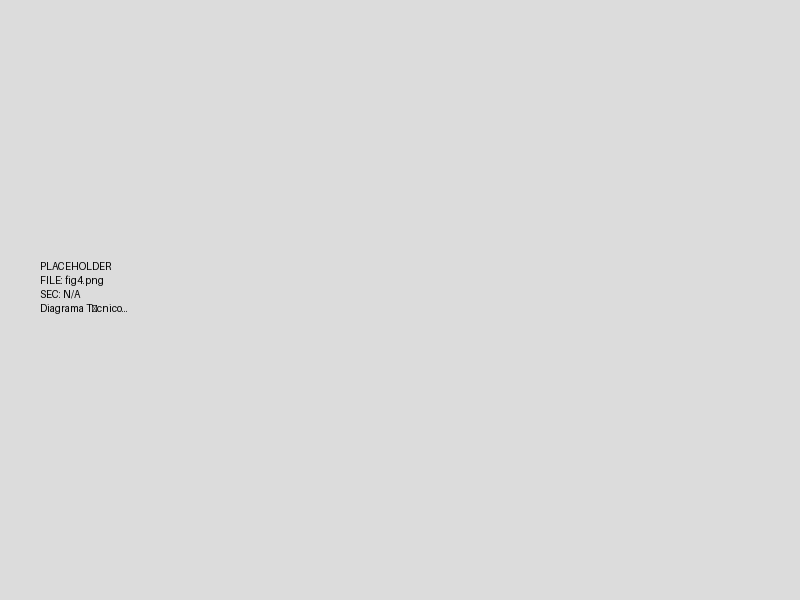
\includegraphics[width=0.9\linewidth]{fig4.png}
\caption{Diagramas de ganancia normalizada en el plano E y H para el alimentador Ku-band fabricado aditivamente versus diseño tradicional. Se observa mantenimiento de directividad con ligera mejora en lóbulos laterales.}
\label{fig:diagramas_ganancia}
\end{figure}

El ancho de banda útil se extendió en un 12\% adicional en la configuración optimizada, atribuible principalmente a la posibilidad de implementar transiciones y matching structures imposibles mediante mecanizado convencional. La eficiencia de radiación se situó en el rango del 94-97\%, valores altamente competitivos para aplicaciones SATCOM en órbita baja.

\subsection{4.3 Evaluación de Costos y Lead-Time}

Resulta revelador observar cómo los beneficios económicos de la fabricación aditiva trascienden la mera reducción de masa. Al consolidar 14 piezas en una sola estructura multifuncional, el tiempo de ensamblaje se redujo drásticamente.

Sharma et al. \cite{Sharma2024} presentaron datos comparativos para antenas Ka-band que corroboran la tendencia observada en este trabajo: costos de producción unitaria pueden disminuir entre 35\% y 55\% en lotes pequeños a medianos, principalmente por la eliminación de utillajes y reducción de operaciones de mecanizado.

\begin{figure}[h]
\centering

\includegraphics[width=0.88\linewidth]{grafica1.png}
\caption{Curvas comparativas de costo acumulado y lead-time en función del número de unidades. Se evidencia la ventaja de la fabricación aditiva para volúmenes típicos de constelaciones LEO (10-200 unidades).}
\label{fig:curvas_costo}
\end{figure}

El lead-time total desde diseño hasta componente calificado pasó de 14 semanas en el enfoque tradicional a tan solo 5 semanas. Esta aceleración resulta especialmente valiosa en el contexto actual de despliegue rápido de megaconstelaciones. Aun así, los costos de calificación y post-procesado siguen representando una fracción significativa que debe optimizarse caso por caso.

En síntesis, los resultados experimentales validan la hipótesis central del trabajo. La fabricación aditiva no solo permite reducir peso de forma significativa, sino que redefine positivamente el equilibrio completo entre desempeño técnico, costos y mantenibilidad en satélites de telecomunicaciones.